\section{Instantaneous Rates of Change: The Derivative}\label{sec:derivative}

A common amusement park ride lifts riders to a height then allows them to freefall a certain distance before safely stopping them. Suppose such a ride drops riders from a height of 150 feet. Students of physics may recall that the height (in feet) of the riders, $t$ seconds after freefall (and ignoring air resistance, etc.) can be accurately modeled by $f(t) = -16t^2+150$. 

Using this formula, it is easy to verify that, without intervention, the riders will hit the ground at $t=2.5\sqrt{1.5} \approx 3.06$ seconds. Suppose the designers of the ride decide to begin slowing the riders' fall after 2 seconds (corresponding to a height of 86 ft.). How fast will the riders be traveling at that time?\\

We have been given a \textit{position} function, but what we want to compute is a velocity at a specific point in time, i.e., we want an \textit{instantaneous velocity}. We do not currently know how to calculate this.

However, we do know from common experience how to calculate an \textit{average velocity}. (If we travel 60 miles in 2 hours, we know we had an average velocity of 30 mph.) We looked at this concept in \autoref{sec:limit_intro} when we introduced the difference quotient. We have 
	$$\frac{\text{change in distance}}{\text{change in time}} = \frac{\text{``\ rise\ ''}}{\text{run}} = \text{average velocity}.$$
	
We can approximate the instantaneous velocity at $t=2$ by considering the average velocity over some time period containing $t=2$. If we make the time interval small, we will get a good approximation. (This fact is commonly used. For instance, high speed cameras are used to track fast moving objects. Distances are measured over a fixed number of frames to generate an accurate approximation of the velocity.)

Consider the interval from $t=2$ to $t=3$ (just before the riders hit the ground). On that interval, the average velocity is 
		$$\frac{f(3)-f(2)}{3-2} = \frac{f(3)-f(2)}{1} =-80\ \text{ft/s},$$
where the minus sign indicates that the riders are moving \textit{down}. By narrowing the interval we consider, we will likely get a better approximation of the instantaneous velocity. On $[2,2.5]$ we have 
	$$\frac{f(2.5)-f(2)}{2.5-2} = \frac{f(2.5)-f(2)}{0.5} =-72\ \text{ft/s}.$$

We can do this for smaller and smaller intervals of time. For instance, over a time span of 1/10$^\text{th}$ of a second, i.e., on $[2,2.1]$, we have 
$$\frac{f(2.1)-f(2)}{2.1-2} = \frac{f(2.1)-f(2)}{0.1} =-65.6\ \text{ft/s}.$$

Over a time span of 1/100$^\text{th}$ of a second, on $[2,2.01]$, the average velocity is
$$\frac{f(2.01)-f(2)}{2.01-2} = \frac{f(2.01)-f(2)}{0.01} =-64.16\ \text{ft/s}.$$

What we are really computing is the average velocity on the interval $[2,2+h]$ for small values of $h$. That is, we are computing $$\frac{f(2+h) - f(2)}{h}$$ where $h$ is the change in time after $2$ seconds.

What we really want is for $h=0$, but this, of course, returns the familiar ``$0/0$'' %\zerooverzero\ 
indeterminate form. So we employ a limit, as we did in \autoref{sec:limit_intro}.

\mtable{Approximating the instantaneous velocity with average velocities over a small time period $h$.}{table:falling}%
{\noindent\begin{tabular}{lc}		
	$h$ & \parbox[b]{75pt}{\centering Average Velocity\par ft/s}\\ \midrule
	$1$ & \makebox[3em][l]{$-80$} \\
	$0.5$ & \makebox[3em][l]{$-72$} \\
	$0.1$ & \makebox[3em][l]{$-65.6$} \\
	$0.01$ & \makebox[3em][l]{$-64.16$} \\
	$0.001$ & \makebox[3em][l]{$-64.016$}
\end{tabular}}

We can approximate the value of this limit numerically with small values of $h$ as seen in \autoref{table:falling}. It looks as though the velocity is approaching $-64$ ft/s. Computing the limit directly gives
\begin{align*}\lim_{h\to 0} \frac{f(2+h)-f(2)}{h}
 &= \lim_{h\to 0}\frac{-16(2+h)^2+150 - (-16(2)^2+150)}{h} \\
 &=	\lim_{h\to 0}\frac{-64h-16h^2}{h} \\
 &= \lim_{h\to 0}-64 -16h \\
 &=-64.
\end{align*}

\mtable{Computing the difference quotient.}{fig:diff_quotient}{\begin{tikzpicture}
\begin{axis}[tick label style={font=\scriptsize},minor x tick num=1,
axis y line=middle,axis x line=middle,ymin=-50,ymax=160,xmin=-.5,xmax=3.49,
name=myplot, extra x ticks={2.4}, extra x tick labels={\begin{tabular}{c}$\uparrow$\\$2+h$\end{tabular}},width=\marginparwidth]
\addplot [{\colorone},domain=0:3.5,thick] {150-16*x*x};
\addplot [{\colortwo},domain=1:3.5,thick] {(90.75-28.16*x)/.4};
\draw[{\colorthree}] (axis cs:2,0)--(axis cs:2,86);
\draw[{\colorthree}] (axis cs:2.4,0)--(axis cs:2.4,57.84); 
\draw[gray] (axis cs:2,25)--(axis cs:2.4,25) node[pos=0.5, below]{\scriptsize $h$};
\node[label={180:{\scriptsize $(2,f(2))$}},circle,fill,inner sep=1pt] at (axis cs:2,86) {};
\node[label={180:{\scriptsize $(2+h,f(2+h))$}},circle,fill,inner sep=1pt] at (axis cs:2.4,57.84) {};
%\node[label={90:{\begin{tabular}{c}\scriptsize $(2+h,f(2+h))$\\$\Big\downarrow$\end{tabular}}},circle,fill,inner sep=1pt] at (axis cs:2.4,57.84) {};
%\node[label={270:{\scriptsize $2+h$}},circle,fill,inner sep=0pt] at (axis cs:2.4,0) {};
\end{axis}
\node [right] at (myplot.right of origin) {\scriptsize $x$};
\node [above] at (myplot.above origin) {\scriptsize $y$};
\end{tikzpicture}}

Graphically, we can view the average velocities we computed numerically as the slopes of secant lines on the graph of $f$ going through the points $(2,f(2))$ and $(2+h,f(2+h))$, as in \autoref{fig:diff_quotient}. In \autoref{fig:derivfalling}, the secant line corresponding to $h=1$ is shown in three contexts. \autoref{fig:derivfalling}(a) shows a ``zoomed out'' version of $f$ with its secant line. In (b), we zoom in around the points of intersection between $f$ and the secant line. Notice how well this secant line approximates $f$ between those two points -- it is a common practice to approximate functions with straight lines.

As $h\to 0$, these secant lines approach the \textit{tangent line}, a line that goes through the point $(2,f(2))$ with the special slope of $-64$. In parts (c) and (d) of \autoref{fig:derivfalling}, we zoom in around the point $(2,86)$. In (c) we see the secant line, which approximates $f$ well, but not as well the tangent line shown in (d).

\begin{figure}[!ht]
%	\flushinner
	\caption{Parts (a), (b) and (c) show the secant line to $f(x)$ with $h=1$, zoomed in different amounts. Part (d) shows the tangent line to $f$ at $x=2$.}\label{fig:derivfalling}
\end{figure}

We have just introduced a number of important concepts that we will flesh out more within this section. First, we formally define two of them.

\definition{def:derivative_at_a_point}{Derivative at a Point}{Let $f$ be a continuous function on an open interval $I$ and let $c$ be in $I$.\index{derivative!at a point} The \sword{derivative of $f$ at $c$}, denoted $\fp(c)$, is \[\lim_{h\to 0}\frac{f(c+h)-f(c)}{h},\] provided the limit exists.}

If the limit exists, we say that \sword{$f$ is differentiable at $c$}; if the limit does not exist, then \sword{$f$ is not differentiable at $c$}. If $f$ is differentiable at every point in $I$, then \sword{$f$ is differentiable on $I$}.\index{differentiable}

\definition{def:tangent_line}{Tangent Line}{Let $f$ be continuous on an open interval $I$ and differentiable at $c$, for some $c$ in $I$. The line with equation $\ell(x) = \fp(c)(x-c)+f(c)$ is the \textbf{tangent line} to the graph of $f$ at $c$; that is, it is the line through $(c,f(c))$ whose slope is the derivative of $f$ at $c$.\index{tangent line}\index{derivative!tangent line}}

\jmtVideo{1O5NEI8UuHM}{the-difference-quotient-example-1}{The Difference Quotient --- Example 1}

Some examples will help us understand these definitions.

\example{ex_derv_point1}{Finding derivatives and tangent lines}{Let $f(x) = 3x^2+5x-7$. Find: 

\noindent\begin{minipage}[t]{.5\textwidth}
	\begin{enumerate}
	\item		$\fp(1)$
	\item		The equation of the tangent line to the graph of $f$ at $x=1$.
	\end{enumerate}
	\end{minipage}%
	\noindent\begin{minipage}[t]{.5\textwidth}
	\begin{enumerate}\addtocounter{enumi}{2}
	\item		$\fp(3)$
	\item		The equation of the tangent line to the graph $f$ at $x=3$.
	\end{enumerate}
	\end{minipage}}%
{	\begin{enumerate}
	\item We compute this directly using \autoref{def:derivative_at_a_point}.
		\begin{align*}
			\fp(1) &= \lim_{h\to 0} \frac{f(1+h)-f(1)}{h} \\
				   &= \lim_{h\to 0} \frac{3(1+h)^2+5(1+h)-7 - (3(1)^2+5(1)-7)}{h}\\
		%\end{align*}
		%\begin{align*}
				   &= \lim_{h\to 0} \frac{3h^2+11h}{h}\\
				   &= \lim_{h\to 0} 3h+11=11.%\\
				   %&= 11.
		\end{align*}
	\item The tangent line at $x=1$ has slope $\fp(1)$ and goes through the point $(1,f(1)) = (1,1)$. Thus the tangent line has equation, in point-slope form, $y = 11(x-1) + 1$. In slope-intercept form we have $y = 11x-10$.
	\item Again, using the definition,
		\begin{align*}
			\fp(3) &= \lim_{h\to 0} \frac{f(3+h)-f(3)}{h} \\
				   &= \lim_{h\to 0} \frac{3(3+h)^2+5(3+h)-7 - (3(3)^2+5(3)-7)}{h} \\
				   &= \lim_{h\to 0} \frac{3h^2+23h}{h}\\
				   &= \lim_{h\to 0} 3h+23 \\
				   &= 23.
		\end{align*}
	\item The tangent line at $x=3$ has slope $23$ and goes through the point $(3,f(3)) = (3,35)$. Thus the tangent line has equation $y=23(x-3)+35 = 23x-34$.
	\end{enumerate}

\mfigure{0in}{A graph of $f(x) = 3x^2+5x-7$ and its tangent lines at $x=1$ and $x=3$.}{fig:tangent1}{figures/figtangent1}

A graph of $f$ is given in \autoref{fig:tangent1} along with the tangent lines at $x=1$ and $x=3$.}

%Another important line that can be created using information from the der\-iv\-ative is the \sword{normal line.} It is perpendicular to the tangent line, hence its slope is the opposite--reciprocal of the tangent line's slope.
%
%\definition{def:normal_line}{Normal Line}
%{Let $f$ be continuous on an open interval $I$ and differentiable at $c$, for some $c$ in $I$. The \textbf{normal line} to the graph of $f$ at $c$ is the line with equation
%\[n(x) =\frac{-1}{\fp(c)}(x-c)+f(c),\] where $\fp(c)\neq 0$. When $\fp(c)=0$, the normal line is the vertical line through $\big(c,f(c)\big)$; that is, $x=c$.\index{derivative!normal line}\index{normal line}
%}
%
%\example{ex_normal1}{Finding equations of normal lines}{Let $f(x) = 3x^2+5x-7$, as in \autoref{ex_derv_point1}. Find the equations of the normal lines to the graph of $f$ at $x=1$ and $x=3$.
%}
%{In \autoref{ex_derv_point1}, we found that $\fp(1)=11$. Hence at $x=1$, the normal line will have slope $-1/11$. An equation for the normal line is $$n(x) = \frac{-1}{11}(x-1)+1.$$
%The normal line is plotted with $y=f(x)$ in \autoref{fig:normal1}. Note how the line looks perpendicular to $f$. (A key word here is ``looks.'' Mathematically, we say that the normal line \emph{is} perpendicular to $f$ at $x=1$ as the slope of the normal line is the opposite--reciprocal of the slope of the tangent line. However, normal lines may not always \emph{look} perpendicular. The aspect ratio of the picture of the graph plays a big role in this.)
%\mfigure{0in}{A graph of $f(x)=3x^2+5x-7$, along with its normal line at $x=1$.}{fig:normal1}{figures/fignormal1}
%
%We also found that $\fp(3) = 23$, so the normal line to the graph of $f$ at $x=3$ will have slope $-1/23$. An equation for the normal line is $$n(x) = \frac{-1}{23}(x-3)+35.$$}

Linear functions are easy to work with; many functions that arise in the course of solving real problems are not easy to work with. A common practice in mathematical problem solving is to approximate difficult functions with not--so--difficult functions. Lines are a common choice. It turns out that at any given point on the graph of a differentiable function $f$, the best linear approximation to $f$ is its tangent line. That is one reason we'll spend considerable time finding tangent lines to functions.

One type of function that does not benefit from a tangent--line approximation is a line; it is rather simple to recognize that the tangent line to a line is the line itself. We look at this in the following example.

\example{ex_der_line}{Finding the Derivative of a Line}{Consider $f(x) = 3x+5$. Find the equation of the tangent line to $f$ at $x=1$ and $x=7$.}
{We find the slope of the tangent line by using \autoref{def:derivative_at_a_point}.

	\begin{align*}
	\fp(1) &=	\lim_{h\to 0}\frac{f(1+h)-f(1)}{h} \\
					&=	\lim_{h\to 0} \frac{3(1+h)+5 - (3+5)}{h}\\
					&=	\lim_{h\to 0} \frac{3h}{h}\\
					&=	\lim_{h\to 0} 3\\
					&= 3.
	\end{align*}
	
We just found that $\fp(1) = 3$. That is, we found the \textit{instantaneous rate of change} of $f(x) = 3x+5$ is $3$. This is not surprising; lines are characterized by being the \textit{only} functions with a \textit{constant rate of change.} That rate of change is called the \textit{slope} of the line. Since their rates of change are constant, their \textit{instantaneous} rates of  change are always the same; they are all the slope.

So given a line $f(x) = ax+b$, the derivative at any point $x$ will be $a$; that is, $\fp(x) = a$. 

It is now easy to see that the tangent line to the graph of $f$ at $x=1$ is just $f$, with the same being true for $x=7$.}

We often desire to find the tangent line to the graph of a function without knowing the actual derivative of the function. In these cases, the best we may be able to do is approximate the tangent line. We demonstrate this in the next example.\\
\mfigure{0in}{$f(x) = \sin x$ graphed with an approximation to its tangent line at $x=0$.}{fig:tangentsinx}{figures/figtangentsinx}

\example{ex_der_num_approx}{Numerical Approximation of the Tangent Line}{Approximate the equation of the tangent line to the graph of $f(x)=\sin x$ at $x=0$.}
{In order to find the equation of the tangent line, we need a slope and a point. The point is given to us: $(0,\sin 0) = (0,0)$. To compute the slope, we need the derivative. This is where we will make an approximation. Recall that $$\fp(0) \approx \frac{\sin(0+h)- \sin 0}{h}$$ for a small value of $h$. We choose (somewhat arbitrarily) to let $h=0.1$. Thus $$\fp(0) \approx \frac{\sin(0.1)-\sin 0}{0.1} \approx 0.9983.$$
Thus our approximation of the equation of the tangent line is $y = 0.9983(x-0) +0 = 0.9983x$; it is graphed in \autoref{fig:tangentsinx}. The graph seems to imply the approximation is rather good.}

Recall from \autoref{sec:limit_analytically} that $\ds \lim_{x\to 0}\frac{\sin x}x =1$, meaning for values of $x$ near 0, $\sin x \approx x$. Since the slope of the line $y=x$ is 1 at $x=0$, it should seem reasonable that ``the slope of $f(x)=\sin x$'' is near 1 at $x=0$. In fact, since we \textit{approximated} the value of the slope to be $0.9983$, we might guess the \textit{actual value} is 1. We'll come back to this later.\bigskip

Consider again \autoref{ex_derv_point1}. To find the derivative of $f$ at $x=1$, we needed to evaluate a limit. To find the derivative of $f$ at $x=3$, we needed to again evaluate a limit. We have this process:
\[
\begin{tabular}{c}input specific\\number $c$\end{tabular}
\longrightarrow
\fbox{\begin{tabular}{c}do something\\to $f$ and $c$\end{tabular}}
\longrightarrow
\begin{tabular}{c}return\\number $\fp(c)$\end{tabular}
\]

This process describes a \textit{function}; given one input (the value of $c$), we return exactly one output (the value of $\fp(c)$). The ``do something'' box is where the tedious work (taking limits) of this function occurs. 

Instead of applying this function repeatedly for different values of $c$, let us apply it just once to the variable $x$. We then take a limit just once. The process now looks like:
\[
\text{input variable x}
\longrightarrow
\fbox{\begin{tabular}{c}do something\\to $f$ and $x$\end{tabular}}
\longrightarrow
\begin{tabular}{c}return\\function $\fp(x)$\end{tabular}
\]

The output is the ``derivative function,'' $\fp(x)$. The $\fp(x)$ function will take a number $c$ as input and return the derivative of $f$ at $c$. This calls for a definition.

%\setlength{\specialboxlength}{\textwidth-10pt}
\definition{def:the_derivative}{Derivative Function}
{Let $f$ be a differentiable function on an open interval $I$. The function $$\fp(x) = \lim_{h\to 0} \frac{f(x+h)-f(x)}{h}$$ is \sword{the derivative of $f$}.\index{derivative!as a function}\index{derivative!notation}\\

\sword{Notation:} 

Let $y = f(x)$. The following notations all represent the derivative:
\[\fp(x)\ =\ y\primeskip'\ =\ \frac{dy}{dx}\ =\ \frac{df}{dx}\ =\ \frac{d}{dx}(f)\ =\ \frac{d}{dx}(y).\]}
%\setlength{\specialboxlength}{\textwidth-2\specialboxinnerseplength}

\paragraph{Important: } The notation $\ds \frac{dy}{dx}$ is one symbol; it is \textbf{not} the fraction ``$dy/dx$''. The notation, while somewhat confusing at first, was chosen with care. A fraction--looking symbol was chosen because the derivative has many fraction--like properties. Among other places, we see these properties at work when we talk about the units of the derivative, when we discuss the Chain Rule, and when we learn about integration (topics that appear in later sections and chapters).\bigskip

Examples will help us understand this definition.

\example{ex_deriv1}{Finding the derivative of a function}{Let $f(x) = 3x^2+5x-7$ as in \autoref{ex_derv_point1}. Find $\fp(x)$.}
{We apply \autoref{def:the_derivative}.
\begin{align*}
	\fp(x)
	&= \lim_{h\to 0} \frac{f(x+h)-f(x)}{h} \\
	&=	\lim_{h\to 0} \frac{3(x+h)^2+5(x+h)-7-(3x^2+5x-7)}{h}\\
	&=	\lim_{h\to 0} \frac{3h^2 +6xh+5h}{h}\\
	&= \lim_{h\to 0} 3h+6x+5\\
	&= 6x+5
\end{align*}
So $\fp(x) = 6x+5$. Recall earlier we found that $\fp(1) = 11$ and $\fp(3) = 23$. Note our new computation of $\fp(x)$ affirm these facts.}

\example{ex_deriv2}{Finding the derivative of a function}{Let $\ds f(x) = \frac{1}{x+1}$. Find $\fp(x)$.}
{We apply \autoref{def:the_derivative}.
\begin{align*}
	\fp(x)
	&= \lim_{h\to 0} \frac{f(x+h)-f(x)}{h}\\
	&=	\lim_{h\to 0} \frac{\frac{1}{x+h+1}-\frac{1}{x+1}}{h}
	\intertext{Now find a common denominator and subtract; factor $1/h$ out front to facilitate reading.}
	\fp(x)
	&= \lim_{h\to 0} \frac{1}{h}\cdot\left(\frac{x+1}{(x+1)(x+h+1)} - \frac{x+h+1}{(x+1)(x+h+1)}\right)\\
	&=	\lim_{h\to 0} \frac 1h\cdot\left(\frac{x+1-(x+h+1)}{(x+1)(x+h+1)}\right)\\
	&=	\lim_{h\to 0} \frac1h\cdot\left(\frac{-h}{(x+1)(x+h+1)}\right)\\
	&=	\lim_{h\to 0} \frac{-1}{(x+1)(x+h+1)} \\
	&= \frac{-1}{(x+1)(x+1)}\\
	&= \frac{-1}{(x+1)^2}
\end{align*}
	
So $\ds\fp(x) = \frac{-1}{(x+1)^2}$. To practice using our notation, we could also state
\[\frac{d}{dx}\left(\frac{1}{x+1}\right) = \frac{-1}{(x+1)^2}.\eoehere\]}

\example{ex_deriv_sinx}{Finding the derivative of a function}{Find the derivative of $f(x) = \sin x$.}
{Before applying \autoref{def:the_derivative}, note that once this is found, we can find the actual tangent line to $f(x) = \sin x$ at $x=0$, whereas we settled for an approximation in \autoref{ex_der_num_approx}. 
	\small
	\begin{align*}
		\fp(x)
		&= \lim_{h\to 0} \frac{\sin(x+h)-\sin x}{h} & & \left(\text{\scriptsize \parbox{110pt}{\centering Use trig identity $\sin(x+h) = \sin x\cos h+\cos x\sin h$}}\right) \\
		&= \lim_{h\to 0} \frac{\sin x\cos h+\cos x\sin h-\sin x}{h} & & \text{\scriptsize (regroup)}\\
		&= \lim_{h\to 0} \frac{\sin x(\cos h-1) + \cos x\sin h}{h} & & \text{\scriptsize (split into two fractions)}\\
		&= \lim_{h\to 0} \left(\frac{\sin x(\cos h-1)}{h} + \frac{\cos x\sin h}{h}\right) & & \left(\text{\scriptsize use $\ds \lim_{h\to 0} \frac{\cos h-1}{h} = 0$ and $\ds \lim_{h\to 0} \frac{\sin h}{h} = 1$}\right)\\
		&=	\sin x\cdot 0 + \cos x \cdot 1 \\
		&= \cos x\ .\eoehere
	\end{align*}}

We have found that when $f(x) = \sin x$, $\fp(x) = \cos x$ (see \autoref{fig:sin_and_dsin}).

\begin{lxfigure}
\centering
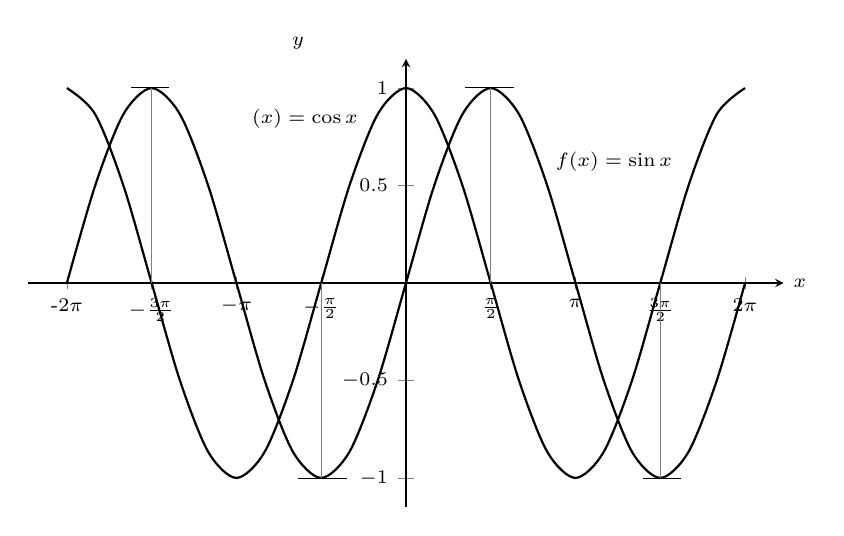
\begin{tikzpicture}
\begin{axis}[tick label style={font=\scriptsize}, axis y line=middle,axis x line=middle, ymin=-1.15, ymax=1.15,xmin=-7,xmax=7,name=myplot,  xtick={-6.28318, -4.7123889, -3.14159, -1.5708, 1.5708, 3.14159, 4.7123889, 6.28318}, xticklabels={-$2\pi$, $-\frac{3\pi}{2}$,$-\pi$, $-\frac{\pi}{2}$, $\frac{\pi}{2}$,$\pi$, $\frac{3\pi}{2}$, $2\pi$}, xscale=1.4]
\addplot [{\colorone}, smooth, domain=-6.28318:6.28318,thick] {sin(deg(x))} 
         node [pos=.7, above right] {\scriptsize $f(x)=\sin{x}$};
\addplot [{\colortwo},smooth, domain=-6.28318:6.28318,thick] {cos(deg(x))}
         node [pos=.45, above left] {\scriptsize $\fp(x)=\cos{x}$};
\draw[\colortwo] (axis cs:-5.1,1.005)--(axis cs:-4.4,1.005);
\draw[\colortwo] (axis cs:-2,-1.005)--(axis cs:-1.1,-1.005);
\draw[\colortwo] (axis cs:5.1,-1.005)--(axis cs:4.4,-1.005);
\draw[\colortwo] (axis cs:2,1.005)--(axis cs:1.1,1.005);  
\draw[gray] (axis cs:-4.7123889,0)--(axis cs:-4.7123889,1);
\draw[gray] (axis cs:-1.5708,0)--(axis cs:-1.5708,-1);
\draw[gray] (axis cs:1.5708,0)--(axis cs:1.5708,1);
\draw[gray] (axis cs:4.7123889,0)--(axis cs:4.7123889,-1);
\end{axis}
\node [right] at (myplot.right of origin) {\scriptsize $x$};
\node [above] at (myplot.above origin) {\scriptsize $y$};
\end{tikzpicture}
\caption{The function $f(x)=\sin x$ and its derivative $\fp(x)=\cos x$.}
\label{fig:sin_and_dsin}
\end{lxfigure}

Initially, this might be somewhat surprising; the result of a tedious limit process and the sine function is a nice function. Then again, perhaps this is not entirely surprising. The sine function is periodic --- it repeats itself on regular intervals. Therefore its rate of change also repeats itself on the same regular intervals. In fact, if we think about $\fp(x)$ as the slope of the tangent to the sine curve we notice the following
\begin{itemize}
\item when the slope of tangent lines is 0 then $\fp(x)=\cos x$ crosses the $x-$axis;
\item when the slopes of the tangent lines are positive then $\fp$ lies above the $x-$axis; and 
\item when the slopes of the tangent lines are negative then $\fp$ lies below the $x-$axis.
\end{itemize}

We should have known the derivative would be periodic; we now know exactly which periodic function it is.

Thinking back to \autoref{ex_der_num_approx}, we can find the slope of the tangent line to $f(x)=\sin x$ at $x=0$ using our derivative. We approximated the slope as $0.9983$; we now know the slope is \textit{exactly} $\cos 0 =1$.

\clearpage

\example{ex_not_diff}{Finding the derivative of a piecewise defined function}{Find the derivative of the absolute value function,
\[f(x) = \abs{x} = \begin{cases}-x & x<0 \\ x & x\geq 0\end{cases}.\]
See \autoref{fig:absolutevalue}.}
{We need to evaluate $\ds \lim_{h\to0}\frac{f(x+h)-f(x)}{h}.$ As $f$ is piecewise-defined, we need to consider separately the limits when $x<0$ and when $x>0$. \\

\mfigure{0in}{The absolute value function, $f(x) = \abs{x}$. Notice how the slope of the lines (and hence the tangent lines) abruptly changes at $x=0$.}{fig:absolutevalue}{figures/figabsolutevalue}

When $x<0$:
	\begin{align*}
	\frac{d}{dx}\big(-x\big)
	&= \lim_{h\to 0}\frac{-(x+h) - (-x)}{h} \\
	&=	\lim_{h\to 0}\frac{-h}{h}\\
	&=	\lim_{h\to 0}-1 \\
	&=	-1.
	\end{align*}
When $x>0$, a similar computation shows that $\ds \frac{d}{dx}\big(x\big) = 1$. \\

We need to also find the derivative at $x=0$. By the definition of the derivative at a point, we have $$\fp(0) = \lim_{h\to0}\frac{f(0+h)-f(0)}{h}.$$ Since $x=0$ is the point where our function's definition switches from one piece to the other, we need to consider left and right-hand limits. Consider the following, where we compute the left and right hand limits side by side.\\
\begin{minipage}[b]{.49\linewidth}
\begin{align*}
\lim_{h\to0^-}\frac{f(0+h)-f(0)}{h} &= \\
\lim_{h\to0^-}\frac{-h-0}{h} &= \\
\lim_{h\to0^-}-1 & =-1
\end{align*}
\end{minipage}\rule{.5pt}{70pt}%
\begin{minipage}[b]{.49\linewidth}
\begin{align*}
\lim_{h\to0^+}\frac{f(0+h)-f(0)}{h} &= \\
\lim_{h\to0^+}\frac{h-0}{h} &= \\
\lim_{h\to0^+}1 & =1
\end{align*}
\end{minipage}
%		
%		$$\begin{array}{ccccc}
%		\displaystyle \lim_{h\to0}\frac{f(0+h)-f(0)}{h} & = & \displaystyle\lim_{h\to0^-}\frac{f(0+h)-f(0)}{h} &=&\displaystyle\lim_{h\to0^+}\frac{f(0+h)-f(0)}{h}\\
%	\rule{0pt}{20pt}	&= & \displaystyle\lim_{h\to0^-}\frac{-h-0}{h} &=&\displaystyle\lim_{h\to0^+}\frac{h-0}{h}\\
%	\rule{0pt}{15pt}	&= & \displaystyle\lim_{h\to0^-}-1 &=&\displaystyle\lim_{h\to0^+}1\\
%	\rule{0pt}{12pt}	&= & -1 &=& 1\\
%		\end{array}$$
%		
\mfigure{-1in}{A graph of the derivative of $f(x) = \abs{x}$.}{fig:absolutevalueprime}{figures/figabsolutevalueprime}

\noindent
The last lines of each column tell the story: the left and right hand limits are not equal. Therefore the limit does not exist at 0, and $f$ is not differentiable at 0; see \autoref{fig:absolutevalueprime}.
So we have $$\fp(x) = \begin{cases} -1 & x<0 \\ 1 & x>0\end{cases}.$$ 
At $x=0$, $\fp(x)$ does not exist; there is a jump discontinuity at 0. So $f(x) = \abs{x}$ is differentiable everywhere except at 0.}

The point of non-differentiability came where the piecewise defined function switched from one piece to the other. Our next example shows that this does not always cause trouble.\bigskip

\example{ex_diff_piecewise}{Finding the derivative of a piecewise defined function}{Find the derivative of $f(x)$, where $\ds f(x) = \begin{cases}\sin x & x\leq \pi/2 \\ 1 & x>\pi/2 \end{cases}.$ See \autoref{fig:piecewisesinx1}.}
{Using \autoref{ex_deriv_sinx}, we know that when $x<\pi/2$, $\fp(x) = \cos x$. It is easy to verify that when $x>\pi/2$, $\fp(x) = 0$; consider:
\mfigure{0in}{A graph of $f(x)$ as defined in \autoref{ex_diff_piecewise}.}{fig:piecewisesinx1}{figures/figpiecewisesinx1}
\[
 \lim_{h\to0}\frac{f(x+h) - f(x)}{h}
 = \lim_{h\to0}\frac{1-1}{h} = \lim_{h\to0}0 =0.
\]

So far we have $$\fp(x) = \begin{cases}\cos x & x<\pi/2\\ 0 & x>\pi/2\end{cases}.$$ We still need to find $\fp(\pi/2)$. Notice at $x=\pi/2$ that both pieces of $\fp$ are 0, meaning we can state that $\fp(\pi/2)=0$. 

Being more rigorous, we can again evaluate the difference quotient limit at $x=\pi/2$, utilizing again left and right--hand limits:\\

\small
\noindent\begin{minipage}{.59\linewidth}
\begin{align*}
\lim_{h\to0^-}\frac{f(\pi/2+h)-f(\pi/2)}{h} &=\\
\lim_{h\to0^-}\frac{\sin(\pi/2+h)-\sin(\pi/2)}{h}&=\\
\lim_{h\to0^-}{ \frac{\sin(\frac{\pi}{2})\cos(h)+\sin(h)\cos(\frac{\pi}{2})-\sin(\frac{\pi}{2})}{h}}&=\\
\lim_{h\to0^-}\frac{1\cdot\cos(h)+\sin(h)\cdot 0-1}{h} &=\\
0
\end{align*}
\end{minipage}
\begin{minipage}{1pt}
 \rule{.5pt}{100pt}
\end{minipage}
\begin{minipage}{.39\linewidth}
\begin{align*}
\lim_{h\to0^+}\frac{f(\pi/2+h)-f(\pi/2)}{h} &=\\
\lim_{h\to0^+}\frac{1-1}{h}&=\\
\lim_{h\to0^+}\frac{0}{h}&=\\
0&\\
\phantom{0}\\
\phantom{0}
\end{align*}
\end{minipage}
\normalsize

%$\ds \lim_{h\to0}\frac{f(\pi/2+h)-f(\pi/2)}{h}=$
%\begin{align*}
% \lim_{h\to0^-}\frac{f(\pi/2+h)-f(\pi/2)}{h}
% &=\lim_{h\to0^+}\frac{f(\pi/2+h)-f(\pi/2)}{h}\\
% \lim_{h\to0^-}\frac{\sin(\pi/2+h)-\sin(\pi/2)}{h} &=\lim_{h\to0^+}\frac{1-1}{h}\\
% \lim_{h\to0^-}{ \frac{\sin(\pi/2)\cos(h)+\sin(h)\cos(\pi/2)-\sin(\pi/2)}{h}}
% &=\lim_{h\to0^+}\frac{0}{h}\\
% \lim_{h\to0^-}\frac{1\cdot\cos(h)+\sin(h)\cdot 0-1}{h} &=\lim_{h\to0^+}0\\
% 0 &=0\\
%\end{align*}
\mfigure{0in}{A graph of $\fp(x)$ in \autoref{ex_diff_piecewise}.}{fig:piecewisecosx1}{figures/figpiecewisecosx1}
Since both the left and right hand limits are 0 at $x=\pi/2$, the limit exists and $\fp(\pi/2)$ exists (and is 0). Therefore we can fully write $\fp$ as $$\fp(x) = \begin{cases}\cos x & x\leq\pi/2\\ 0 & x>\pi/2\end{cases}.$$ See \autoref{fig:piecewisecosx1} for a graph of this function.}

Recall we pseudo-defined a continuous function as one in which we could sketch its graph without lifting our pencil. We can give a pseudo--definition for differentiability as well: it is a continuous function that does not have any ``sharp corners.'' One such sharp corner is shown in \autoref{fig:absolutevalue}. Even though the function $f$ in \autoref{ex_diff_piecewise} is piecewise--defined, the transition is ``smooth'' hence it is differentiable. Note how in the graph of $f$ in \autoref{fig:piecewisesinx1} it is difficult to tell when $f$ switches from one piece to the other; there is no ``corner.''

\ifthenelse{\boolean{latexml}}{%
 To better understand the definition of a derivative, experiment with the Geogebra app at \url{http://mathinsight.org/applet/secant_line_slope}.%
% todo Tim : iframe ?
}{%
 \exvideo{%
  \begin{minipage}[t]{2cm}%
   \vspace{-.5\baselineskip}\qrcode{http://mathinsight.org/applet/secant_line_slope}%
  \end{minipage}
  \quad
  \begin{minipage}[t]{.74\linewidth}%
   To better understand the definition of a derivative, experiment with the Geogebra app at \\
   \url{http://mathinsight.org/applet/secant_line_slope}.%
  \end{minipage}%
 }%
}

This section defined the derivative; in some sense, it answers the question of ``What \textit{is} the derivative?'' The next section addresses the question ``What does the derivative \textit{mean}?''


\printexercises{exercises/02_01_exercises}
